CrowdNote was developed as a classic Web system. To facilitate the sharing of all produced software, only technologies that do not require complex infrastructure were adopted. The Server was fully developed in NodeJS for easy deployment, the Client was developed in HTML 5 to improve compatibility, and the Database uses MongoDB as No-SQL database for flexible persistence.

The architecture of the CrowdNote is illustrated in Figure~\ref{architecture} in which is possible observe the 3 main components: Server, Database, and Clients.

\begin{figure}[h!]
	\centerline{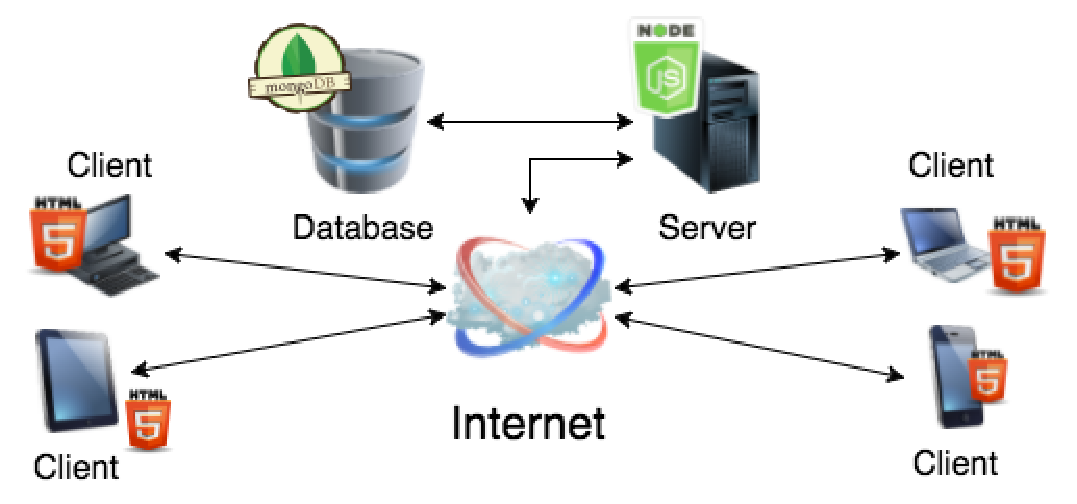
\includegraphics[scale=0.3] {figure/Architecture}}
	\caption{CrowdNote Architecture}
	\label{architecture}
\end{figure}


\subsection{The Server Component}
The server system, illustrated in Figure~\ref{server}, is composed of 3 modules: Collector, Aggregator and Player Provider.

\begin{figure}[h!]
	\centerline{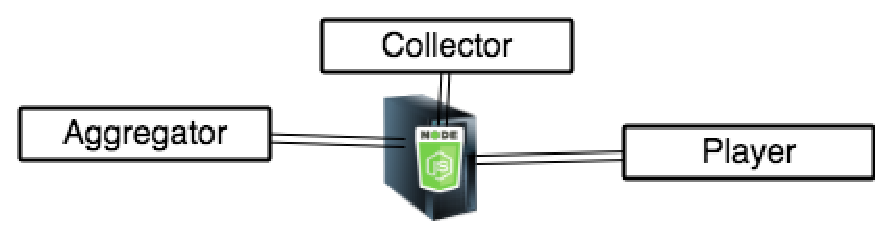
\includegraphics[scale=0.4] {figure/server}}
	\caption{Server Component}
	\label{server}
\end{figure}

\begin{itemize}

\item \textbf{Collector: } The Collector sends the jobs to the workers, receives the annotations from them, and stores the annotations into the Database.

\item \textbf{Aggregator: } Aggregator verifies, filters, groups, and processes the collected annotations of the crowd according to the rules defined for each task, and then stores the result in the Database.

\item \textbf{Player Provider: } The Player Provider sends to the client the annotations, the extra content, and the original video. Thus, the player on the client can play the enriched video synchronously.

\end{itemize}

\subsection{The Database Component}
The persistence was addressed using MongoDB, which delivers a very attractive solution to build No-SQL databases with some characteristics that meet the crowdsourcing requirements such as high write load, high availability in an unreliable environment,  easy scaling and partition, heterogeneous data into the same collection.

In this model, JSON document collections are used instead of tables, and the documents in each collection may have a different structure to store different attributes. This feature allowed the modeling of a very simple database structure, composed of 3 collections of documents, as can be seen in Figure~\ref{persistence}. It was possible because documents in the Input and Output collections can contain different fields according to the task that consumes or generates the entries.

The Video collection stores entries related to the video segments dataset, the Input collection stores the input entries to the tasks, and the Output collection stores the contributions collected from the crowd.

\begin{figure}[h]
	\centerline{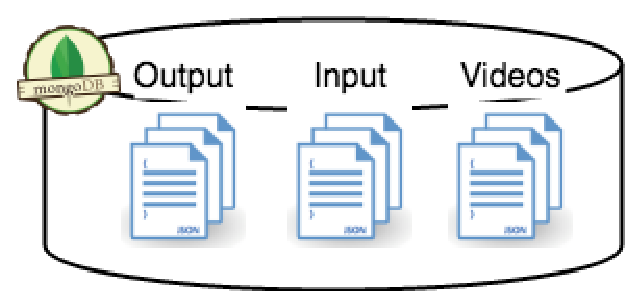
\includegraphics[scale=0.3] {figure/Persistence}}
	\caption{No-SQL Database - JSON Documents Collections}
	\label{persistence}
\end{figure}

The result of the aggregation for each task is stored in the Input collection to be used by the next task, supporting the cascading tasks approach.

\subsection{The Client Component}
The client consists of simple forms-based annotation tools and a player capable of playing video content and content synchronously. The client has been fully developed in HTML5, in the simplest way possible. For each task, a simple annotation tool was created to collect contributions.



\subsection{Workflow}
The 3 main components of CrowdNote communicate through data flows from \textbf{A} to \textbf{G}, as can be seen in the workflow in Figure~\ref{workflow}.

\begin{figure}[h]
	\centerline{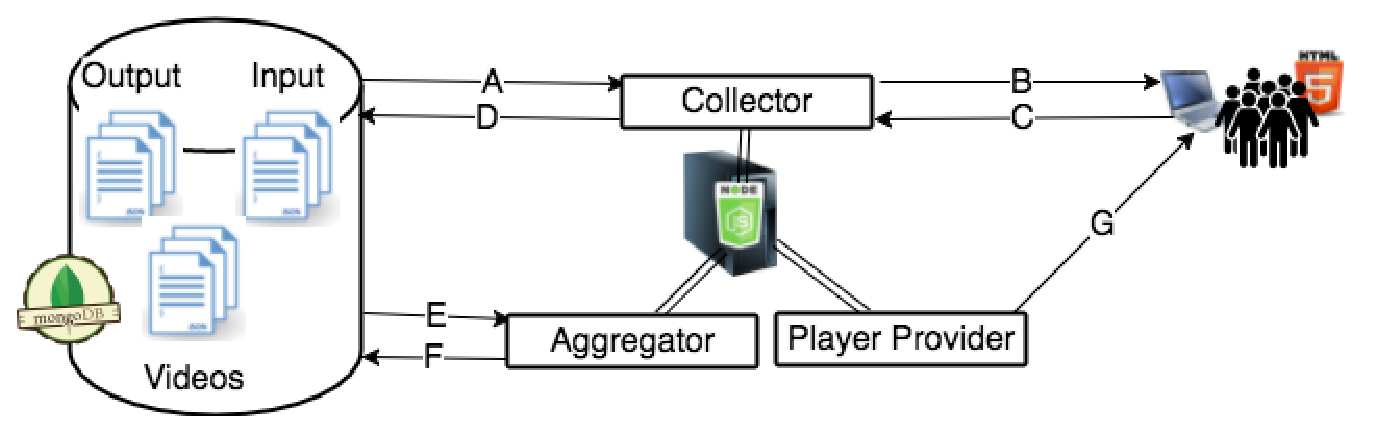
\includegraphics[scale=0.36] {figure/Workflow}}
	\caption{CrowdNote Workflow}
	\label{workflow}
\end{figure}

\begin{itemize}
\item \textbf{A:} To generate each job to be sent to a worker, the Collector receives an entry from the Input Collection and the corresponding entry from the Videos Collection.

\item \textbf{B:} The Collector sends a job to an instance of the Client, to be executed by a worker.

\item \textbf{C:} The Client sends to the Collector the annotation made by the worker for the work received.

\item \textbf{D:} The Collector stores in the Output collection the annotation collected from a worker.

\item \textbf{E:} The Aggregator receives from the Output collection all annotations collected for a given task.

\item \textbf{F:} The aggregator stores the resulting entries from the aggregation process in the Input collection so that they are supplied as input to the next task.

\item \textbf{G:} The outcome of the cascade of microtasks is sent by the Player Provider to the client so that it can play the video synchronously with the extra content.
\end{itemize}
